\documentclass[11pt,a4paper]{article}
\usepackage[margin=2cm]{geometry}
\usepackage[T1]{fontenc}
\usepackage[utf8]{inputenc}
\usepackage{array}
\usepackage{longtable}
\usepackage{enumitem}
\usepackage{hyperref}
\usepackage{tikz}
\usepackage{xurl}
\usetikzlibrary{arrows.meta, positioning, shapes.geometric}
\setlist{nosep}
\setlength{\emergencystretch}{3em}
\sloppy
\hypersetup{colorlinks=true, linkcolor=blue, urlcolor=blue}

\title{PDF and IFC Workflow Report}
\author{Mid Term 1 Accessibility Checking Prototype}
\date{12 June 2026}

\begin{document}
\maketitle

\section{Flow Diagram}

\begin{center}
\resizebox{0.98\textwidth}{0.70\textheight}{%
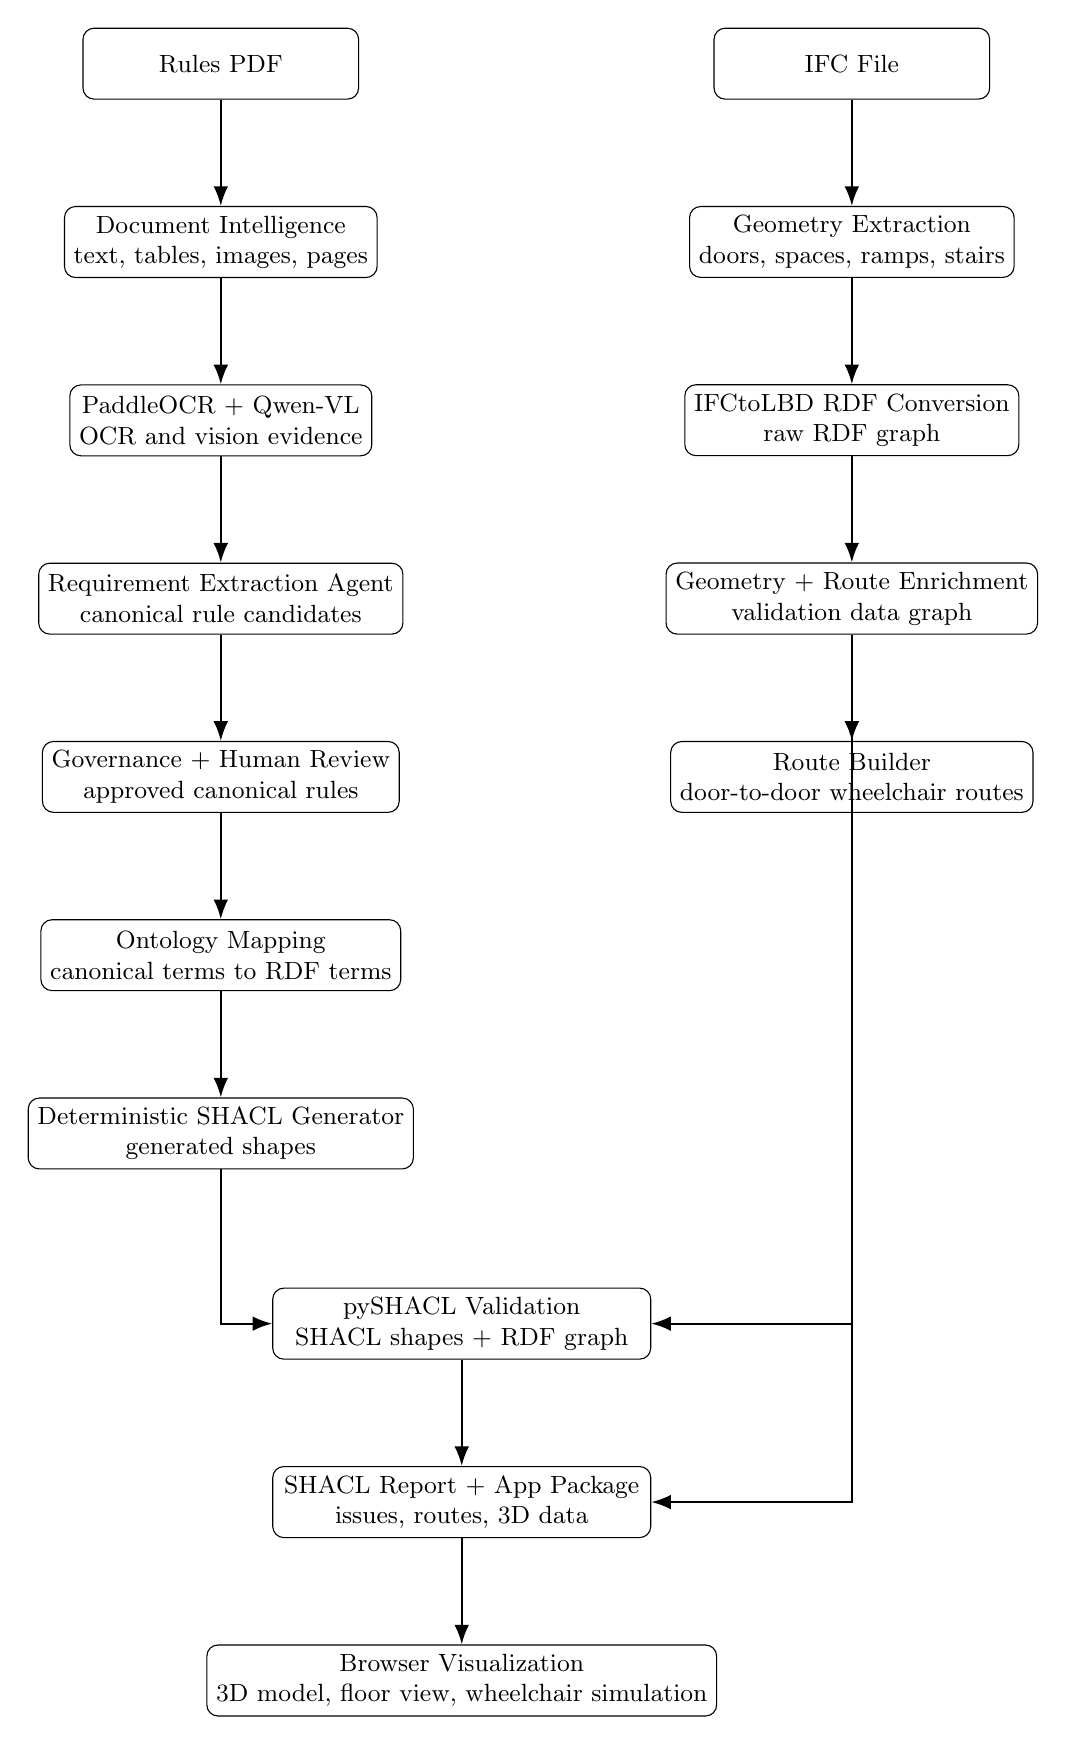
\begin{tikzpicture}[
  node distance=1.35cm and 2.2cm,
  box/.style={rectangle, draw, rounded corners, align=center, minimum width=3.5cm, minimum height=0.9cm, font=\small},
  wide/.style={rectangle, draw, rounded corners, align=center, minimum width=4.8cm, minimum height=0.9cm, font=\small},
  arrow/.style={-{Latex[length=2.5mm]}, thick}
]
\node[box] (pdf) {Rules PDF};
\node[box, below=of pdf] (di) {Document Intelligence\\text, tables, images, pages};
\node[box, below=of di] (ocrvision) {PaddleOCR + Qwen-VL\\OCR and vision evidence};
\node[box, below=of ocrvision] (extract) {Requirement Extraction Agent\\canonical rule candidates};
\node[box, below=of extract] (gov) {Governance + Human Review\\approved canonical rules};
\node[box, below=of gov] (map) {Ontology Mapping\\canonical terms to RDF terms};
\node[box, below=of map] (shacl) {Deterministic SHACL Generator\\generated shapes};

\node[box, right=4.5cm of pdf] (ifc) {IFC File};
\node[box, below=of ifc] (geom) {Geometry Extraction\\doors, spaces, ramps, stairs};
\node[box, below=of geom] (rdf) {IFCtoLBD RDF Conversion\\raw RDF graph};
\node[box, below=of rdf] (enrich) {Geometry + Route Enrichment\\validation data graph};
\node[box, below=of enrich] (route) {Route Builder\\door-to-door wheelchair routes};

\node[wide, below right=1.5cm and -1.8cm of shacl] (validate) {pySHACL Validation\\SHACL shapes + RDF graph};
\node[wide, below=of validate] (report) {SHACL Report + App Package\\issues, routes, 3D data};
\node[wide, below=of report] (browser) {Browser Visualization\\3D model, floor view, wheelchair simulation};

\draw[arrow] (pdf) -- (di);
\draw[arrow] (di) -- (ocrvision);
\draw[arrow] (ocrvision) -- (extract);
\draw[arrow] (extract) -- (gov);
\draw[arrow] (gov) -- (map);
\draw[arrow] (map) -- (shacl);
\draw[arrow] (ifc) -- (geom);
\draw[arrow] (geom) -- (rdf);
\draw[arrow] (rdf) -- (enrich);
\draw[arrow] (enrich) -- (route);
\draw[arrow] (shacl) |- (validate);
\draw[arrow] (enrich) |- (validate);
\draw[arrow] (route) |- (report);
\draw[arrow] (validate) -- (report);
\draw[arrow] (report) -- (browser);
\end{tikzpicture}
}
\end{center}

\section{Short Explanation}

The system receives two files:

\begin{itemize}
  \item \textbf{IFC file}: the building model, for example \texttt{AC20-Institute-Var-2.ifc}.
  \item \textbf{Rules PDF}: the rule book or standard, for example \texttt{planungsgrundlagen\_barrierefreies\_bauen.pdf}.
\end{itemize}

The two files move through separate pipelines first. The PDF becomes approved canonical rules and then SHACL constraints. The IFC becomes an RDF graph with geometry and route data. Both sides meet at pySHACL validation.

\section{Step-by-Step File Journey}

\begin{longtable}{|p{1.2cm}|p{3.5cm}|p{4.2cm}|p{6.3cm}|}
\hline
\textbf{Step} & \textbf{Component} & \textbf{File or data entering} & \textbf{What happens} \\
\hline
1 & \texttt{preprocess.py} & IFC file and rules PDF & This is the main runner. It sends the IFC into the building workflow and the PDF into the rule extraction workflow. Output is written to \texttt{output/app\_package/}. \\
\hline
2 & Geometry extraction & IFC file & The system reads doors, spaces, walls, stairs, ramps, slabs, and columns. It extracts positions, bounding boxes, widths, heights, floor levels, labels, and IFC IDs. \\
\hline
3 & IFCtoLBD & IFC file & The IFC model is converted into RDF. RDF stores facts as graph triples, for example that one object is an \texttt{IfcDoor}. Output: \texttt{raw\_lbd\_graph.ttl}. \\
\hline
4 & RDF enrichment & Raw RDF graph and geometry objects & The system adds measured values to the RDF graph, such as door width, ramp slope, clear route width, and turning space. Output: \texttt{lbd\_graph.ttl}. \\
\hline
5 & Route builder & IFC geometry and spaces & The system builds wheelchair route edges, such as door-to-door paths. It records route width, door width, turning space, ramp data, and stair intersections. \\
\hline
6 & 3D package writer & Elements, routes, and issues & The system prepares browser files such as \texttt{app\_data.json}, \texttt{route\_model.glb}, and \texttt{route\_graph.bin}. \\
\hline
7 & Document Intelligence & Rules PDF & The PDF is split into text chunks, table chunks, image chunks, and page metadata. It also renders full pages and table regions as images, so vector diagrams and page-drawn tables can be seen. \\
\hline
8 & PaddleOCR & Embedded images, rendered pages, rendered table regions & OCR means text recognition from images. PaddleOCR reads visible text from image evidence and attaches the result to each image chunk. \\
\hline
9 & Image ranking & All image chunks with OCR and page context & Every image chunk is scored using general evidence signals: measurement density, numeric density, normative language, OCR text quality, page context, table context, visual size, and uniqueness. \\
\hline
10 & Vision model & Top-ranked image chunks & Qwen-VL looks at selected images and writes observations about visible measurements, diagrams, labels, tables, limits, and ranges. \\
\hline
11 & Requirement Extraction Agent & Text, tables, OCR text, and vision observations & The agent extracts canonical rule candidates. It must output neutral rule objects only. It is not allowed to output SHACL, RDF, or ontology mappings. \\
\hline
12 & Candidate governance & Canonical rule candidates & The system compares candidates, detects duplicates, checks conflicts, and chooses the best-supported candidate using evidence quality. \\
\hline
13 & Human review & Selected rules and mapping candidates & Rules cannot become SHACL automatically. A reviewer, timestamp, rationale, and decision must exist before publication. \\
\hline
14 & Ontology mapping & Approved canonical rules and RDF graph & The system maps neutral rule terms to RDF properties. For example, a canonical ramp-width rule maps to the RDF property that stores ramp usable width. \\
\hline
15 & SHACL generator & Approved rules and approved mappings & Python templates generate SHACL deterministically. No LLM generates SHACL. Output: \texttt{generated\_accessibility\_rules.shacl.ttl}. \\
\hline
16 & pySHACL validation & Generated SHACL and enriched RDF graph & pySHACL checks whether the building graph satisfies the generated SHACL constraints. Output: \texttt{shacl\_report.ttl}. \\
\hline
17 & Issue conversion & SHACL report, elements, and routes & SHACL validation results are converted into app issue records, such as route too narrow, ramp too steep, or turning space too small. \\
\hline
18 & Browser frontend & App package files & The browser shows the 3D model, floors, routes, wheelchair simulation, issue list, and SHACL report data. The browser is only a viewer. Compliance is decided by pySHACL. \\
\hline
\end{longtable}

\section{PDF Pipeline In Simple Form}

\begin{verbatim}
Rules PDF
  -> Document Intelligence
  -> text chunks, table chunks, embedded images,
     rendered full pages, rendered table regions
  -> PaddleOCR
  -> image ranking
  -> Qwen-VL vision
  -> requirement extraction agent
  -> canonical rule candidates
  -> governance selection
  -> human review
  -> ontology mapping
  -> deterministic SHACL generation
  -> generated SHACL file
\end{verbatim}

\section{IFC Pipeline In Simple Form}

\begin{verbatim}
IFC file
  -> geometry extraction
  -> IFCtoLBD RDF conversion
  -> geometry and route enrichment
  -> route graph generation
  -> validation data graph
\end{verbatim}

\section{Where Both Pipelines Meet}

\begin{verbatim}
Generated SHACL file + validation data graph
  -> pySHACL
  -> SHACL report
  -> app_data.json
  -> browser visualization and wheelchair simulation
\end{verbatim}

\section{Important Notes}

\begin{itemize}
  \item The PDF pipeline now sees more than embedded images. It also sees rendered pages and rendered table regions.
  \item This helps when a PDF contains diagrams, table lines, arrows, or measurements that are drawn directly on the page.
  \item The SHACL generator is deterministic. It uses Python templates, not an LLM.
  \item The browser does not decide compliance. It only displays the prepared result.
  \item The system is stronger now, but it is not production-perfect. In the latest audit, \texttt{door\_width} was still missing from the final canonical rules.
\end{itemize}

\section{Main Output Files}

\begin{longtable}{|p{6.4cm}|p{8.3cm}|}
\hline
\textbf{File} & \textbf{Purpose} \\
\hline
\path{output/app_package/document_chunks.json} & Structured PDF output: pages, text, tables, image evidence, OCR text, vision text, and ranking metadata. \\
\hline
\path{output/app_package/canonical_rules.json} & Extracted canonical rules from the PDF. \\
\hline
\path{output/app_package/rule_extraction_audit.json} & Evidence, model calls, accepted outputs, rejected outputs, and retrieval audit. \\
\hline
\path{output/app_package/rule_review.json} & Human review records for rules and mappings. \\
\hline
\path{output/app_package/ontology_mappings.json} & Mapping from canonical rule terms to RDF classes and properties. \\
\hline
\path{output/app_package/generated_accessibility_rules.shacl.ttl} & Generated deterministic SHACL shapes. \\
\hline
\path{output/app_package/lbd_graph.ttl} & RDF graph used as validation data. \\
\hline
\path{output/app_package/shacl_report.ttl} & pySHACL validation report. \\
\hline
\path{output/app_package/app_data.json} & Browser data: building elements, routes, issues, and simulation data. \\
\hline
\path{output/app_package/route_model.glb} & 3D model used by the browser. \\
\hline
\end{longtable}

\end{document}
